\graphicspath{{./figures/5-hyperblock-scheduling/}}

\chapter{Evaluation}%
\label{sec:evaluation}%
\label{sec:performance-comparison}

The evaluation aims to answer the following research questions:

\begin{enumerate}[label=\textbf{RQ\arabic*}]
\item Is Vericert competitive with unverified HLS tools?
\item Does adding scheduling to Vericert lead to a significant improvement in
  the quality of the generated hardware (in terms of area and delay)?
\item Is hyperblock scheduling better than na\"ive list scheduling?
\item Did the design decisions (e.g. \cref{sec:thirdattempt}) lead to an
  acceptable compilation time?
\item How effective is the correctness theorem in Vericert?
\end{enumerate}

\section{Experimental Setup}

\def\polybench{PolyBench/C}

\paragraph{Choice of HLS tool for comparison.} \vericert{} is compared against
Bambu HLS 2023.1~\cite{ferrandi21_bambu}, because it is open-source and hence
easily accessible, but still produces hardware
\textquote[{\textcite{pilato13_bambu}}]{produce faster accelerators in almost
  all the cases} compared to LegUp HLS, which is said to produce hardware
\textquote[{\textcite{canis11_legup}}]{of comparable quality to a commercial
  high-level synthesis tool}.  The baseline Bambu HLS version has all the
default automatic optimisations turned on.  \vericert{} is also compared against
an unoptimised version of Bambu HLS, where all optimisations that can be toggled
are turned off.  This affects optimisations like deep if-conversion that Bambu
HLS would normally automatically perform.  Additionally, three versions of
Vericert are compared to Bambu HLS, so that optimisations performed by Vericert
can also be tested.  The first version of Vericert is disables scheduling
completely, generating sequential hardware where an instruction is executed
every clock cycle.  Next, a version of Vericert with list scheduling is
implemented by disabling if-conversion, thereby only scheduling basic blocks.
Finally, a version of Vericert with the full hyperblock scheduling optimisation
is shown, including all optimisations that are implemented.

\paragraph{Choice and preparation of benchmarks.} I xevaluate \vericert{} using
the \polybench{} benchmark suite (version 4.2.1)~\cite{pouchet20_polyb_c}, which
is a collection of 30 numerical kernels. \polybench{} is popular in the HLS
context~\cite{choi18_hbods,pouchet13_polyh,zhao17_comba,zuo13_improv}, since it
has affine loop bounds, making it attractive for streaming computation on FPGA
architectures.  It was also used as part of
\textcite{six22_formal_verif_super_sched} evaluation of their scheduling
optimisation.  I was able to use 27 of the 30 programs; three had to be
discarded (\texttt{cor\-re\-la\-tion}, \texttt{gram\-schmi\-dt} and
\texttt{de\-riche}) because they involve square roots, requiring floats, which
\vericert{} does not support.  I configured \polybench{}'s parameters so that
only integer types are used and use \polybench{}'s smallest datasets for each
program to ensure that data can reside within on-chip memories of the FPGA,
avoiding any need for off-chip memory accesses. The benchmarks have not been
modified to make them run through Bambu HLS optimally, e.g. by adding pragmas
that trigger more advanced optimisations.

\vericert{} implements divisions and modulo operations in C using the
corresponding built-in Verilog operators. These built-in operators are designed
to complete within a single clock cycle, and this causes substantial penalties
in clock frequency.  Other HLS tools, including LegUp, supply their own
multi-cycle division/modulo implementations, and I plan to do the same in future
versions of \vericert{}.  In the meantime, I have prepared an alternative
version of the benchmarks in which each division/modulo operation is replaced
with my own implementation that uses repeated division and multiplications by 2.
Comparing Vericert against Bambu HLS on benchmarks with division without using
the C implementation of division would be futile, as preliminary tests show that
because of the use of the default combinational divider circuit generated by the
synthesis tool, the maximum clock frequency would achieved by Vericert is around
30$\times$ less than the maximum clock frequency achieved by Bambu, which uses a
pipelined division implementation.  The following comparisons are therefore
performed on a modified version of \polybench{} with divisions replaced with
function calls to our C divider implementation.  The final result produced by
the benchmarks remain unchanged.

\paragraph{Synthesis setup} For each benchmark, the resulting Verilog hardware
design was simulated using Verilator to get the total cycle count.  Each design
was synthesised, placed, and routed onto a Xilinx series 7 FPGA (part number:
\mono{xc7z020clg484-1}) using Vivado 2023.1 to get its total area and its
maximum frequency.  Next, the total execution time was calculated as
$\text{total execution time} = \frac{\text{total clock cycles}}{\text{maximum
    frequency}}$.  I ensured that every design met the timing constraints of a
100MHz clock.

\definecolor{colorVericertBase}{HTML}{66c2a5}
\definecolor{colorVericertList}{HTML}{fc8d62}
\definecolor{colorVericertHyper}{HTML}{8da0cb}
\definecolor{colorBambuNoOpt}{HTML}{e78ac3}
\definecolor{colorBambuDefault}{HTML}{bbbbbb}

\colorlet{colorVericertBaseLIGHT}{colorVericertBase!50!white}
\colorlet{colorVericertListLIGHT}{colorVericertList!50!white}
\colorlet{colorVericertHyperLIGHT}{colorVericertHyper!50!white}
\colorlet{colorBambuNoOptLIGHT}{colorBambuNoOpt!50!white}
\colorlet{colorBambuDefaultLIGHT}{colorBambuDefault!50!white}

\newcommand\BambuDefault{%
\setul{-1pt}{3pt}\setulcolor{colorBambuDefaultLIGHT}%
{\ul{\textsf{Bambu-default}}}}

\newcommand\BambuNoOpt{%
\setul{-1pt}{3pt}\setulcolor{colorBambuNoOptLIGHT}%
{\ul{\textsf{Bambu-no-opt}}}}

\newcommand\VericertBase{%
\setul{-1pt}{3pt}\setulcolor{colorVericertBaseLIGHT}%
{\ul{\textsf{Vericert-no-scheduling}}}}

\newcommand\VericertList{%
\setul{-1pt}{3pt}\setulcolor{colorVericertListLIGHT}%
{\ul{\textsf{Vericert-list-scheduling}}}}

\newcommand\VericertHyper{%
\setul{-1pt}{3pt}\setulcolor{colorVericertHyperLIGHT}%
{\ul{\textsf{Vericert-hyperblock-scheduling}}}}

% \begin{figure}
%   \centering
%   \resizebox{\linewidth}{!}{% GNUPLOT: LaTeX picture with Postscript
\begingroup
  \makeatletter
  \providecommand\color[2][]{%
    \GenericError{(gnuplot) \space\space\space\@spaces}{%
      Package color not loaded in conjunction with
      terminal option `colourtext'%
    }{See the gnuplot documentation for explanation.%
    }{Either use 'blacktext' in gnuplot or load the package
      color.sty in LaTeX.}%
    \renewcommand\color[2][]{}%
  }%
  \providecommand\includegraphics[2][]{%
    \GenericError{(gnuplot) \space\space\space\@spaces}{%
      Package graphicx or graphics not loaded%
    }{See the gnuplot documentation for explanation.%
    }{The gnuplot epslatex terminal needs graphicx.sty or graphics.sty.}%
    \renewcommand\includegraphics[2][]{}%
  }%
  \providecommand\rotatebox[2]{#2}%
  \@ifundefined{ifGPcolor}{%
    \newif\ifGPcolor
    \GPcolortrue
  }{}%
  \@ifundefined{ifGPblacktext}{%
    \newif\ifGPblacktext
    \GPblacktexttrue
  }{}%
  % define a \g@addto@macro without @ in the name:
  \let\gplgaddtomacro\g@addto@macro
  % define empty templates for all commands taking text:
  \gdef\gplbacktext{}%
  \gdef\gplfronttext{}%
  \makeatother
  \ifGPblacktext
    % no textcolor at all
    \def\colorrgb#1{}%
    \def\colorgray#1{}%
  \else
    % gray or color?
    \ifGPcolor
      \def\colorrgb#1{\color[rgb]{#1}}%
      \def\colorgray#1{\color[gray]{#1}}%
      \expandafter\def\csname LTw\endcsname{\color{white}}%
      \expandafter\def\csname LTb\endcsname{\color{black}}%
      \expandafter\def\csname LTa\endcsname{\color{black}}%
      \expandafter\def\csname LT0\endcsname{\color[rgb]{1,0,0}}%
      \expandafter\def\csname LT1\endcsname{\color[rgb]{0,1,0}}%
      \expandafter\def\csname LT2\endcsname{\color[rgb]{0,0,1}}%
      \expandafter\def\csname LT3\endcsname{\color[rgb]{1,0,1}}%
      \expandafter\def\csname LT4\endcsname{\color[rgb]{0,1,1}}%
      \expandafter\def\csname LT5\endcsname{\color[rgb]{1,1,0}}%
      \expandafter\def\csname LT6\endcsname{\color[rgb]{0,0,0}}%
      \expandafter\def\csname LT7\endcsname{\color[rgb]{1,0.3,0}}%
      \expandafter\def\csname LT8\endcsname{\color[rgb]{0.5,0.5,0.5}}%
    \else
      % gray
      \def\colorrgb#1{\color{black}}%
      \def\colorgray#1{\color[gray]{#1}}%
      \expandafter\def\csname LTw\endcsname{\color{white}}%
      \expandafter\def\csname LTb\endcsname{\color{black}}%
      \expandafter\def\csname LTa\endcsname{\color{black}}%
      \expandafter\def\csname LT0\endcsname{\color{black}}%
      \expandafter\def\csname LT1\endcsname{\color{black}}%
      \expandafter\def\csname LT2\endcsname{\color{black}}%
      \expandafter\def\csname LT3\endcsname{\color{black}}%
      \expandafter\def\csname LT4\endcsname{\color{black}}%
      \expandafter\def\csname LT5\endcsname{\color{black}}%
      \expandafter\def\csname LT6\endcsname{\color{black}}%
      \expandafter\def\csname LT7\endcsname{\color{black}}%
      \expandafter\def\csname LT8\endcsname{\color{black}}%
    \fi
  \fi
    \setlength{\unitlength}{0.0500bp}%
    \ifx\gptboxheight\undefined%
      \newlength{\gptboxheight}%
      \newlength{\gptboxwidth}%
      \newsavebox{\gptboxtext}%
    \fi%
    \setlength{\fboxrule}{0.5pt}%
    \setlength{\fboxsep}{1pt}%
    \definecolor{tbcol}{rgb}{1,1,1}%
\begin{picture}(10800.00,7200.00)%
    \gplgaddtomacro\gplbacktext{%
      \csname LTb\endcsname%%
      \put(518,5449){\makebox(0,0)[r]{\strut{}1}}%
      \csname LTb\endcsname%%
      \put(518,5766){\makebox(0,0)[r]{\strut{}2}}%
      \csname LTb\endcsname%%
      \put(518,5951){\makebox(0,0)[r]{\strut{}3}}%
      \csname LTb\endcsname%%
      \put(518,6185){\makebox(0,0)[r]{\strut{}5}}%
      \csname LTb\endcsname%%
      \put(518,6501){\makebox(0,0)[r]{\strut{}10}}%
      \csname LTb\endcsname%%
      \put(518,6920){\makebox(0,0)[r]{\strut{}25}}%
    }%
    \gplgaddtomacro\gplfronttext{%
      \csname LTb\endcsname%%
      \put(161,6202){\rotatebox{-270}{\makebox(0,0){\strut{}Relative execution time}}}%
    }%
    \gplgaddtomacro\gplbacktext{%
      \csname LTb\endcsname%%
      \put(518,3477){\makebox(0,0)[r]{\strut{}1}}%
      \csname LTb\endcsname%%
      \put(518,3811){\makebox(0,0)[r]{\strut{}2}}%
      \csname LTb\endcsname%%
      \put(518,4007){\makebox(0,0)[r]{\strut{}3}}%
      \csname LTb\endcsname%%
      \put(518,4253){\makebox(0,0)[r]{\strut{}5}}%
      \csname LTb\endcsname%%
      \put(518,4587){\makebox(0,0)[r]{\strut{}10}}%
      \csname LTb\endcsname%%
      \put(518,5029){\makebox(0,0)[r]{\strut{}25}}%
    }%
    \gplgaddtomacro\gplfronttext{%
      \csname LTb\endcsname%%
      \put(161,4228){\rotatebox{-270}{\makebox(0,0){\strut{}Relative cycle count}}}%
    }%
    \gplgaddtomacro\gplbacktext{%
      \csname LTb\endcsname%%
      \put(616,1546){\makebox(0,0)[r]{\strut{}0.7}}%
      \csname LTb\endcsname%%
      \put(616,1855){\makebox(0,0)[r]{\strut{}1.0}}%
      \csname LTb\endcsname%%
      \put(616,2455){\makebox(0,0)[r]{\strut{}2.0}}%
      \csname LTb\endcsname%%
      \put(616,2806){\makebox(0,0)[r]{\strut{}3.0}}%
      \csname LTb\endcsname%%
      \put(616,3055){\makebox(0,0)[r]{\strut{}4.0}}%
      \csname LTb\endcsname%%
      \put(888,1448){\rotatebox{-90}{\makebox(0,0)[l]{\strut{}2mm}}}%
      \csname LTb\endcsname%%
      \put(1237,1448){\rotatebox{-90}{\makebox(0,0)[l]{\strut{}3mm}}}%
      \csname LTb\endcsname%%
      \put(1586,1448){\rotatebox{-90}{\makebox(0,0)[l]{\strut{}adi}}}%
      \csname LTb\endcsname%%
      \put(1935,1448){\rotatebox{-90}{\makebox(0,0)[l]{\strut{}atas}}}%
      \csname LTb\endcsname%%
      \put(2284,1448){\rotatebox{-90}{\makebox(0,0)[l]{\strut{}bicg}}}%
      \csname LTb\endcsname%%
      \put(2633,1448){\rotatebox{-90}{\makebox(0,0)[l]{\strut{}cholesky}}}%
      \csname LTb\endcsname%%
      \put(2982,1448){\rotatebox{-90}{\makebox(0,0)[l]{\strut{}covariance}}}%
      \csname LTb\endcsname%%
      \put(3331,1448){\rotatebox{-90}{\makebox(0,0)[l]{\strut{}doitgen}}}%
      \csname LTb\endcsname%%
      \put(3680,1448){\rotatebox{-90}{\makebox(0,0)[l]{\strut{}durbin}}}%
      \csname LTb\endcsname%%
      \put(4029,1448){\rotatebox{-90}{\makebox(0,0)[l]{\strut{}fdtd-2d}}}%
      \csname LTb\endcsname%%
      \put(4378,1448){\rotatebox{-90}{\makebox(0,0)[l]{\strut{}floyd-warshall}}}%
      \csname LTb\endcsname%%
      \put(4727,1448){\rotatebox{-90}{\makebox(0,0)[l]{\strut{}gemm}}}%
      \csname LTb\endcsname%%
      \put(5076,1448){\rotatebox{-90}{\makebox(0,0)[l]{\strut{}gemver}}}%
      \csname LTb\endcsname%%
      \put(5425,1448){\rotatebox{-90}{\makebox(0,0)[l]{\strut{}gesummv}}}%
      \csname LTb\endcsname%%
      \put(5774,1448){\rotatebox{-90}{\makebox(0,0)[l]{\strut{}heat-3d}}}%
      \csname LTb\endcsname%%
      \put(6123,1448){\rotatebox{-90}{\makebox(0,0)[l]{\strut{}jacobi-1d}}}%
      \csname LTb\endcsname%%
      \put(6472,1448){\rotatebox{-90}{\makebox(0,0)[l]{\strut{}jacobi-2d}}}%
      \csname LTb\endcsname%%
      \put(6821,1448){\rotatebox{-90}{\makebox(0,0)[l]{\strut{}lu}}}%
      \csname LTb\endcsname%%
      \put(7170,1448){\rotatebox{-90}{\makebox(0,0)[l]{\strut{}ludcmp}}}%
      \csname LTb\endcsname%%
      \put(7519,1448){\rotatebox{-90}{\makebox(0,0)[l]{\strut{}mvt}}}%
      \csname LTb\endcsname%%
      \put(7868,1448){\rotatebox{-90}{\makebox(0,0)[l]{\strut{}nussinov}}}%
      \csname LTb\endcsname%%
      \put(8217,1448){\rotatebox{-90}{\makebox(0,0)[l]{\strut{}seidel-2d}}}%
      \csname LTb\endcsname%%
      \put(8566,1448){\rotatebox{-90}{\makebox(0,0)[l]{\strut{}symm}}}%
      \csname LTb\endcsname%%
      \put(8915,1448){\rotatebox{-90}{\makebox(0,0)[l]{\strut{}syr2k}}}%
      \csname LTb\endcsname%%
      \put(9264,1448){\rotatebox{-90}{\makebox(0,0)[l]{\strut{}syrk}}}%
      \csname LTb\endcsname%%
      \put(9613,1448){\rotatebox{-90}{\makebox(0,0)[l]{\strut{}trisolv}}}%
      \csname LTb\endcsname%%
      \put(9962,1448){\rotatebox{-90}{\makebox(0,0)[l]{\strut{}trmm}}}%
      \csname LTb\endcsname%%
      \put(10311,1448){\rotatebox{-90}{\makebox(0,0)[l]{\strut{}median}}}%
    }%
    \gplgaddtomacro\gplfronttext{%
      \csname LTb\endcsname%%
      \put(161,2300){\rotatebox{-270}{\makebox(0,0){\strut{}Relative area}}}%
      \csname LTb\endcsname%%
      \put(9730,2896){\makebox(0,0)[r]{\strut{}\footnotesize Vericert-original}}%
      \csname LTb\endcsname%%
      \put(9730,2720){\makebox(0,0)[r]{\strut{}\footnotesize Vericert-list-scheduling}}%
      \csname LTb\endcsname%%
      \put(9730,2545){\makebox(0,0)[r]{\strut{}\footnotesize Vericert-hyperblock-scheduling}}%
      \csname LTb\endcsname%%
      \put(9730,2369){\makebox(0,0)[r]{\strut{}\footnotesize Bambu-no-opt}}%
    }%
    \gplbacktext
    \put(0,0){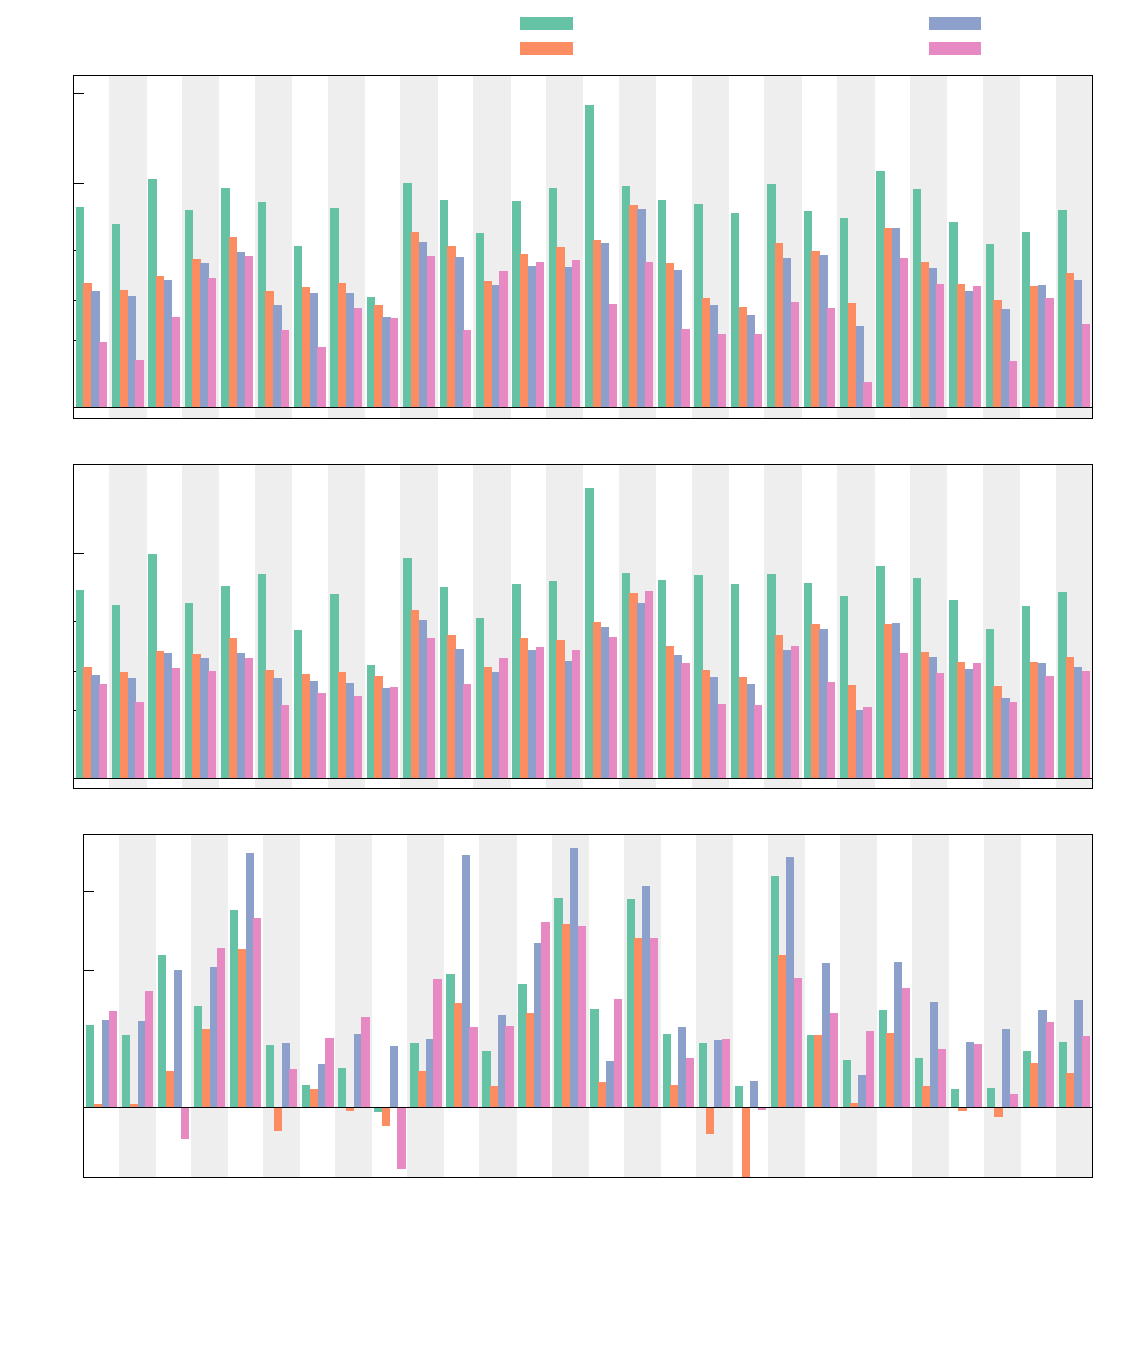
\includegraphics[width={540.00bp},height={360.00bp}]{bar-plot}}%
    \gplfronttext
  \end{picture}%
\endgroup
}
%   \caption[Results of simulating and synthesising the PolyBench/C benchmark suite using a range of HLS tools. All figures are relative to Bambu.]{Results of simulating and synthesising the PolyBench/C benchmark suite using a range of HLS tools. All figures are relative to \BambuDefault{}.}%
%   \label{fig:list-against-hyper-scheduling}
% \end{figure}

\afterpage{
\clearpage% To flush out all floats, might not be what you want
\thispagestyle{empty}
\begin{landscape}
%\thispagestyle{lscape}
%\pagestyle{lscape}
\begin{figure}
  \centering
  \resizebox{\linewidth}{!}{% GNUPLOT: LaTeX picture with Postscript
\begingroup
  \makeatletter
  \providecommand\color[2][]{%
    \GenericError{(gnuplot) \space\space\space\@spaces}{%
      Package color not loaded in conjunction with
      terminal option `colourtext'%
    }{See the gnuplot documentation for explanation.%
    }{Either use 'blacktext' in gnuplot or load the package
      color.sty in LaTeX.}%
    \renewcommand\color[2][]{}%
  }%
  \providecommand\includegraphics[2][]{%
    \GenericError{(gnuplot) \space\space\space\@spaces}{%
      Package graphicx or graphics not loaded%
    }{See the gnuplot documentation for explanation.%
    }{The gnuplot epslatex terminal needs graphicx.sty or graphics.sty.}%
    \renewcommand\includegraphics[2][]{}%
  }%
  \providecommand\rotatebox[2]{#2}%
  \@ifundefined{ifGPcolor}{%
    \newif\ifGPcolor
    \GPcolortrue
  }{}%
  \@ifundefined{ifGPblacktext}{%
    \newif\ifGPblacktext
    \GPblacktexttrue
  }{}%
  % define a \g@addto@macro without @ in the name:
  \let\gplgaddtomacro\g@addto@macro
  % define empty templates for all commands taking text:
  \gdef\gplbacktext{}%
  \gdef\gplfronttext{}%
  \makeatother
  \ifGPblacktext
    % no textcolor at all
    \def\colorrgb#1{}%
    \def\colorgray#1{}%
  \else
    % gray or color?
    \ifGPcolor
      \def\colorrgb#1{\color[rgb]{#1}}%
      \def\colorgray#1{\color[gray]{#1}}%
      \expandafter\def\csname LTw\endcsname{\color{white}}%
      \expandafter\def\csname LTb\endcsname{\color{black}}%
      \expandafter\def\csname LTa\endcsname{\color{black}}%
      \expandafter\def\csname LT0\endcsname{\color[rgb]{1,0,0}}%
      \expandafter\def\csname LT1\endcsname{\color[rgb]{0,1,0}}%
      \expandafter\def\csname LT2\endcsname{\color[rgb]{0,0,1}}%
      \expandafter\def\csname LT3\endcsname{\color[rgb]{1,0,1}}%
      \expandafter\def\csname LT4\endcsname{\color[rgb]{0,1,1}}%
      \expandafter\def\csname LT5\endcsname{\color[rgb]{1,1,0}}%
      \expandafter\def\csname LT6\endcsname{\color[rgb]{0,0,0}}%
      \expandafter\def\csname LT7\endcsname{\color[rgb]{1,0.3,0}}%
      \expandafter\def\csname LT8\endcsname{\color[rgb]{0.5,0.5,0.5}}%
    \else
      % gray
      \def\colorrgb#1{\color{black}}%
      \def\colorgray#1{\color[gray]{#1}}%
      \expandafter\def\csname LTw\endcsname{\color{white}}%
      \expandafter\def\csname LTb\endcsname{\color{black}}%
      \expandafter\def\csname LTa\endcsname{\color{black}}%
      \expandafter\def\csname LT0\endcsname{\color{black}}%
      \expandafter\def\csname LT1\endcsname{\color{black}}%
      \expandafter\def\csname LT2\endcsname{\color{black}}%
      \expandafter\def\csname LT3\endcsname{\color{black}}%
      \expandafter\def\csname LT4\endcsname{\color{black}}%
      \expandafter\def\csname LT5\endcsname{\color{black}}%
      \expandafter\def\csname LT6\endcsname{\color{black}}%
      \expandafter\def\csname LT7\endcsname{\color{black}}%
      \expandafter\def\csname LT8\endcsname{\color{black}}%
    \fi
  \fi
    \setlength{\unitlength}{0.0500bp}%
    \ifx\gptboxheight\undefined%
      \newlength{\gptboxheight}%
      \newlength{\gptboxwidth}%
      \newsavebox{\gptboxtext}%
    \fi%
    \setlength{\fboxrule}{0.5pt}%
    \setlength{\fboxsep}{1pt}%
    \definecolor{tbcol}{rgb}{1,1,1}%
\begin{picture}(14400.00,9360.00)%
    \gplgaddtomacro\gplbacktext{%
      \csname LTb\endcsname%%
      \put(592,6569){\makebox(0,0)[r]{\strut{}1}}%
      \csname LTb\endcsname%%
      \put(592,6987){\makebox(0,0)[r]{\strut{}2}}%
      \csname LTb\endcsname%%
      \put(592,7232){\makebox(0,0)[r]{\strut{}3}}%
      \csname LTb\endcsname%%
      \put(592,7540){\makebox(0,0)[r]{\strut{}5}}%
      \csname LTb\endcsname%%
      \put(592,7958){\makebox(0,0)[r]{\strut{}10}}%
      \csname LTb\endcsname%%
      \put(592,8510){\makebox(0,0)[r]{\strut{}25}}%
    }%
    \gplgaddtomacro\gplfronttext{%
      \csname LTb\endcsname%%
      \put(195,7563){\rotatebox{-270}{\makebox(0,0){\strut{}Relative execution time}}}%
      \csname LTb\endcsname%%
      \put(6685,9124){\makebox(0,0)[r]{\strut{}\small Vericert-original}}%
      \csname LTb\endcsname%%
      \put(6685,8884){\makebox(0,0)[r]{\strut{}\small Vericert-list-scheduling}}%
      \csname LTb\endcsname%%
      \put(10607,9124){\makebox(0,0)[r]{\strut{}\small Vericert-hyperblock-scheduling}}%
      \csname LTb\endcsname%%
      \put(10607,8884){\makebox(0,0)[r]{\strut{}\small Bambu-no-opt}}%
    }%
    \gplgaddtomacro\gplbacktext{%
      \csname LTb\endcsname%%
      \put(592,4004){\makebox(0,0)[r]{\strut{}1}}%
      \csname LTb\endcsname%%
      \put(592,4448){\makebox(0,0)[r]{\strut{}2}}%
      \csname LTb\endcsname%%
      \put(592,4707){\makebox(0,0)[r]{\strut{}3}}%
      \csname LTb\endcsname%%
      \put(592,5034){\makebox(0,0)[r]{\strut{}5}}%
      \csname LTb\endcsname%%
      \put(592,5478){\makebox(0,0)[r]{\strut{}10}}%
      \csname LTb\endcsname%%
      \put(592,6064){\makebox(0,0)[r]{\strut{}25}}%
    }%
    \gplgaddtomacro\gplfronttext{%
      \csname LTb\endcsname%%
      \put(195,5001){\rotatebox{-270}{\makebox(0,0){\strut{}Relative cycle count}}}%
    }%
    \gplgaddtomacro\gplbacktext{%
      \csname LTb\endcsname%%
      \put(692,1649){\makebox(0,0)[r]{\strut{}0.7}}%
      \csname LTb\endcsname%%
      \put(692,2027){\makebox(0,0)[r]{\strut{}1.0}}%
      \csname LTb\endcsname%%
      \put(692,2761){\makebox(0,0)[r]{\strut{}2.0}}%
      \csname LTb\endcsname%%
      \put(692,3191){\makebox(0,0)[r]{\strut{}3.0}}%
      \csname LTb\endcsname%%
      \put(692,3496){\makebox(0,0)[r]{\strut{}4.0}}%
      \csname LTb\endcsname%%
      \put(1030,1548){\rotatebox{-90}{\makebox(0,0)[l]{\strut{}2mm}}}%
      \csname LTb\endcsname%%
      \put(1505,1548){\rotatebox{-90}{\makebox(0,0)[l]{\strut{}3mm}}}%
      \csname LTb\endcsname%%
      \put(1979,1548){\rotatebox{-90}{\makebox(0,0)[l]{\strut{}adi}}}%
      \csname LTb\endcsname%%
      \put(2454,1548){\rotatebox{-90}{\makebox(0,0)[l]{\strut{}atas}}}%
      \csname LTb\endcsname%%
      \put(2928,1548){\rotatebox{-90}{\makebox(0,0)[l]{\strut{}bicg}}}%
      \csname LTb\endcsname%%
      \put(3402,1548){\rotatebox{-90}{\makebox(0,0)[l]{\strut{}cholesky}}}%
      \csname LTb\endcsname%%
      \put(3877,1548){\rotatebox{-90}{\makebox(0,0)[l]{\strut{}covariance}}}%
      \csname LTb\endcsname%%
      \put(4351,1548){\rotatebox{-90}{\makebox(0,0)[l]{\strut{}doitgen}}}%
      \csname LTb\endcsname%%
      \put(4826,1548){\rotatebox{-90}{\makebox(0,0)[l]{\strut{}durbin}}}%
      \csname LTb\endcsname%%
      \put(5300,1548){\rotatebox{-90}{\makebox(0,0)[l]{\strut{}fdtd-2d}}}%
      \csname LTb\endcsname%%
      \put(5775,1548){\rotatebox{-90}{\makebox(0,0)[l]{\strut{}floyd-warshall}}}%
      \csname LTb\endcsname%%
      \put(6249,1548){\rotatebox{-90}{\makebox(0,0)[l]{\strut{}gemm}}}%
      \csname LTb\endcsname%%
      \put(6724,1548){\rotatebox{-90}{\makebox(0,0)[l]{\strut{}gemver}}}%
      \csname LTb\endcsname%%
      \put(7198,1548){\rotatebox{-90}{\makebox(0,0)[l]{\strut{}gesummv}}}%
      \csname LTb\endcsname%%
      \put(7672,1548){\rotatebox{-90}{\makebox(0,0)[l]{\strut{}heat-3d}}}%
      \csname LTb\endcsname%%
      \put(8147,1548){\rotatebox{-90}{\makebox(0,0)[l]{\strut{}jacobi-1d}}}%
      \csname LTb\endcsname%%
      \put(8621,1548){\rotatebox{-90}{\makebox(0,0)[l]{\strut{}jacobi-2d}}}%
      \csname LTb\endcsname%%
      \put(9096,1548){\rotatebox{-90}{\makebox(0,0)[l]{\strut{}lu}}}%
      \csname LTb\endcsname%%
      \put(9570,1548){\rotatebox{-90}{\makebox(0,0)[l]{\strut{}ludcmp}}}%
      \csname LTb\endcsname%%
      \put(10045,1548){\rotatebox{-90}{\makebox(0,0)[l]{\strut{}mvt}}}%
      \csname LTb\endcsname%%
      \put(10519,1548){\rotatebox{-90}{\makebox(0,0)[l]{\strut{}nussinov}}}%
      \csname LTb\endcsname%%
      \put(10993,1548){\rotatebox{-90}{\makebox(0,0)[l]{\strut{}seidel-2d}}}%
      \csname LTb\endcsname%%
      \put(11468,1548){\rotatebox{-90}{\makebox(0,0)[l]{\strut{}symm}}}%
      \csname LTb\endcsname%%
      \put(11942,1548){\rotatebox{-90}{\makebox(0,0)[l]{\strut{}syr2k}}}%
      \csname LTb\endcsname%%
      \put(12417,1548){\rotatebox{-90}{\makebox(0,0)[l]{\strut{}syrk}}}%
      \csname LTb\endcsname%%
      \put(12891,1548){\rotatebox{-90}{\makebox(0,0)[l]{\strut{}trisolv}}}%
      \csname LTb\endcsname%%
      \put(13366,1548){\rotatebox{-90}{\makebox(0,0)[l]{\strut{}trmm}}}%
      \csname LTb\endcsname%%
      \put(13840,1548){\rotatebox{-90}{\makebox(0,0)[l]{\strut{}\bfseries{}median}}}%
    }%
    \gplgaddtomacro\gplfronttext{%
      \csname LTb\endcsname%%
      \put(195,2572){\rotatebox{-270}{\makebox(0,0){\strut{}Relative area}}}%
    }%
    \gplbacktext
    \put(0,0){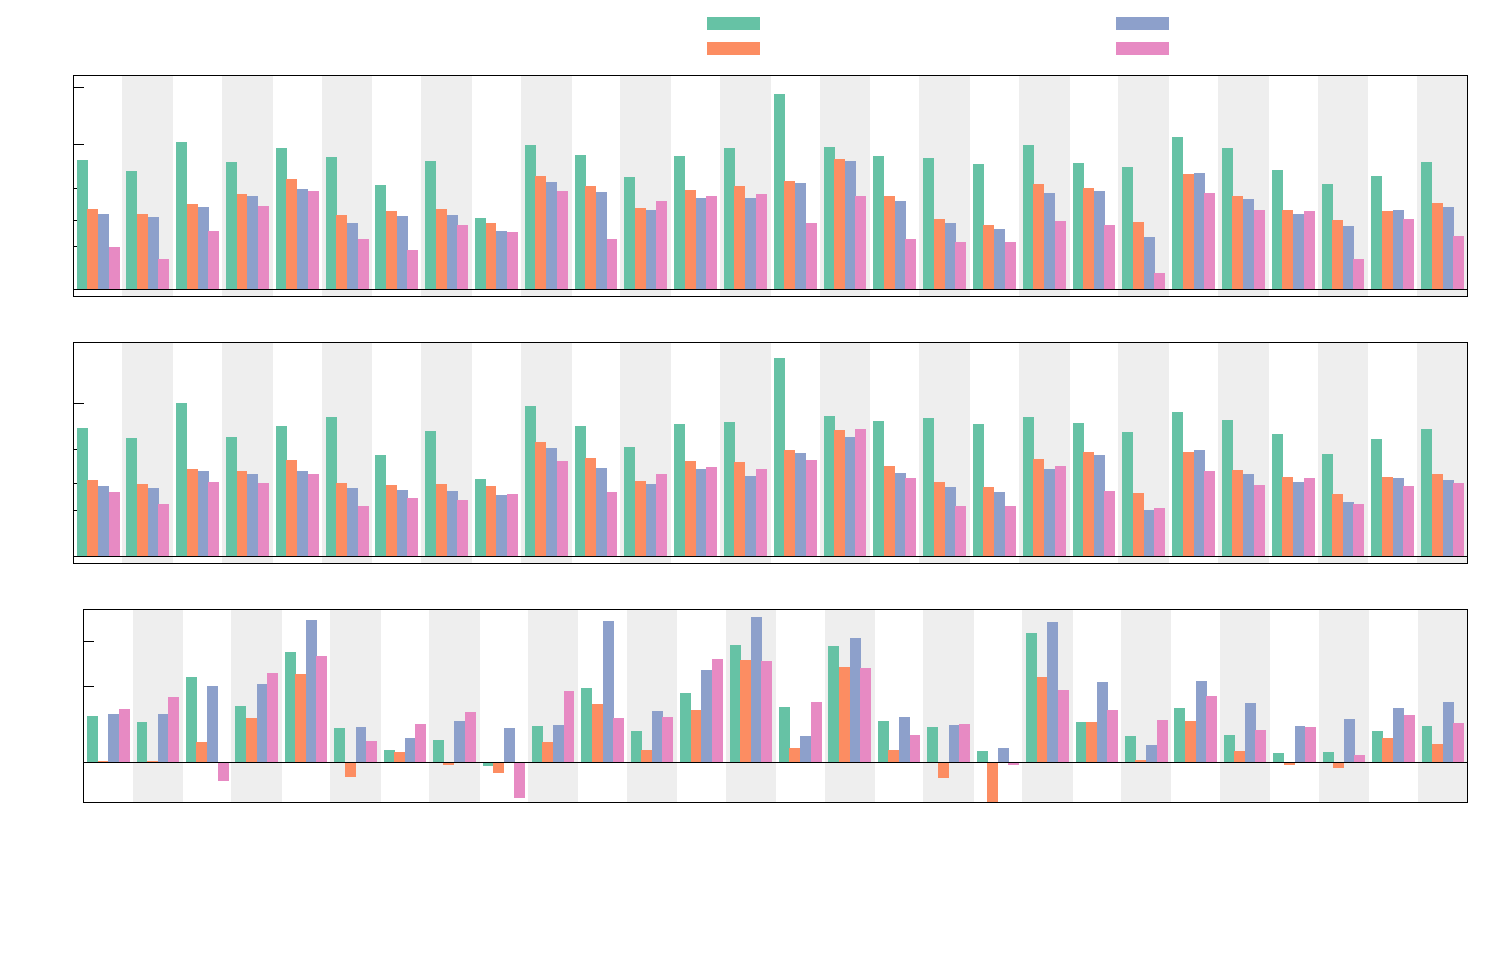
\includegraphics[width={720.00bp},height={468.00bp}]{bar-plot-sideways}}%
    \gplfronttext
  \end{picture}%
\endgroup
}
  \caption[Results of simulating and synthesising the PolyBench/C benchmark
  suite using a range of HLS tools.]{Results of simulating and synthesising the
    PolyBench/C benchmark suite using a range of HLS tools. All figures are
    relative to \BambuDefault{}.}%
\label{fig:list-against-hyper-scheduling}
\end{figure}
\end{landscape}
}

\section{RQ1: Is Vericert Competitive With Unverified Tools}

To assess how \VericertHyper{} fares against unverified HLS tools, I compare it
against the state-of-the-art open-source HLS tool
Bambu~\cite[]{ferrandi21_bambu}. Bambu is used in two modes: one where all
default optimisations are enabled (\BambuDefault{}), and one where as many
optimisations as possible are disabled (\BambuNoOpt{}). Note that several
\enquote{optimisations} are built into Bambu and cannot be disabled, such as
list scheduling and loop flattening.

All the bars in \cref{fig:list-against-hyper-scheduling} are relative to
\BambuDefault. The pink bars show \BambuNoOpt. We see that although
\VericertHyper{} is well behind \BambuDefault{} (its designs require 3$\times$
the cycle count), it performs comparably to \BambuNoOpt{} (1.04$\times$ the
cycle count), which is encouraging because \VericertHyper{} and \BambuNoOpt{}
have similar feature sets.

Comparing the execution time of the hardware designs produced by Vericert
compared to unoptimised Bambu HLS, we see that Vericert designs are around
$1.6\times$ slower than Bambu HLS designs.  This is because Vericert designs
operate normally close to the maximum frequency of 100MHz, whereas Bambu HLS
designs in general seem to give more slack.

Finally, comparing area, on average all tools are quite similar, and Vericert
can achieve designs that are around the same size as optimised Bambu and
unoptimised Bambu.  One thing to note, is that Bambu could be made to optimise
the design purely for area, instead of the default configuration that was
chosen, in which case execution speed might suffer slightly but the area could
be reduced further.

\section{RQ2: Area and Delay Improvements of Vericert}

To assess whether adding scheduling to Vericert leads to better hardware
designs, \cref{fig:list-against-hyper-scheduling} compares the hardware produced
by original Vericert (\VericertBase{}) with that produced when hyperblock
scheduling is enabled (\VericertHyper{}). We see that, on average, hyperblock
scheduling leads to hardware that requires only 0.46$\times$ the cycle count
(middle plot). This is unsurprising given that original Vericert only executed a
single instruction per clock cycle. In terms of area (bottom plot), hyperblock
scheduling has, on average, a slight increase in area.

\section{RQ3: Hyperblock Scheduling Compared to Na\"ive Scheduling}

Hyperblock scheduling is considerably more complicated to implement and verify
than list scheduling, as it requires if-conversion to combine basic blocks into
hyperblocks, as well as predicate-aware scheduling. If we omit if-conversion
entirely (hence avoiding predication too), we obtain list scheduling as a
special case. Does hyperblock scheduling yield enough of a performance
improvement over list scheduling to justify its additional complexity?

To answer this, \cref{fig:list-against-hyper-scheduling} measures the hardware
produced by Vericert with list scheduling (\VericertList{}). On average, list
scheduling leads to hardware that requires 0.51$\times$ the cycle count compared
to \VericertBase{}, which is 1.1$\times$ the cycle count compared to
\VericertHyper{}. I expect hyperblock scheduling to extend its small lead over
list scheduling once the heuristics that guide if-conversion are improved.  In
particular, our predictions of the latency of predicated instructions are
currently quite conservative to ensure that timing constraints are met;
improving these estimates is an active research
area~\cite{tan15_mappin_lut_fpgas,rizzi23_iterat_method_mappin_aware_frequen,wang23_mapbuf,ustun20_accur_fpga_hls,zheng14_fast_effec_placem_routin_direc}.

In terms of area, we see that \VericertList{} leads to the smallest hardware
designs. This can be attributed to the downstream logic synthesis tool being
able to save area by optimising chained operations, such as
multiply--accumulate, while not having to handle the predicates that are
introduced with \VericertHyper{}.

\section{RQ4: Compilation Times of Vericert}

\begin{figure}
  \centering
  \resizebox{\linewidth}{!}{% GNUPLOT: LaTeX picture with Postscript
\begingroup
  \makeatletter
  \providecommand\color[2][]{%
    \GenericError{(gnuplot) \space\space\space\@spaces}{%
      Package color not loaded in conjunction with
      terminal option `colourtext'%
    }{See the gnuplot documentation for explanation.%
    }{Either use 'blacktext' in gnuplot or load the package
      color.sty in LaTeX.}%
    \renewcommand\color[2][]{}%
  }%
  \providecommand\includegraphics[2][]{%
    \GenericError{(gnuplot) \space\space\space\@spaces}{%
      Package graphicx or graphics not loaded%
    }{See the gnuplot documentation for explanation.%
    }{The gnuplot epslatex terminal needs graphicx.sty or graphics.sty.}%
    \renewcommand\includegraphics[2][]{}%
  }%
  \providecommand\rotatebox[2]{#2}%
  \@ifundefined{ifGPcolor}{%
    \newif\ifGPcolor
    \GPcolortrue
  }{}%
  \@ifundefined{ifGPblacktext}{%
    \newif\ifGPblacktext
    \GPblacktexttrue
  }{}%
  % define a \g@addto@macro without @ in the name:
  \let\gplgaddtomacro\g@addto@macro
  % define empty templates for all commands taking text:
  \gdef\gplbacktext{}%
  \gdef\gplfronttext{}%
  \makeatother
  \ifGPblacktext
    % no textcolor at all
    \def\colorrgb#1{}%
    \def\colorgray#1{}%
  \else
    % gray or color?
    \ifGPcolor
      \def\colorrgb#1{\color[rgb]{#1}}%
      \def\colorgray#1{\color[gray]{#1}}%
      \expandafter\def\csname LTw\endcsname{\color{white}}%
      \expandafter\def\csname LTb\endcsname{\color{black}}%
      \expandafter\def\csname LTa\endcsname{\color{black}}%
      \expandafter\def\csname LT0\endcsname{\color[rgb]{1,0,0}}%
      \expandafter\def\csname LT1\endcsname{\color[rgb]{0,1,0}}%
      \expandafter\def\csname LT2\endcsname{\color[rgb]{0,0,1}}%
      \expandafter\def\csname LT3\endcsname{\color[rgb]{1,0,1}}%
      \expandafter\def\csname LT4\endcsname{\color[rgb]{0,1,1}}%
      \expandafter\def\csname LT5\endcsname{\color[rgb]{1,1,0}}%
      \expandafter\def\csname LT6\endcsname{\color[rgb]{0,0,0}}%
      \expandafter\def\csname LT7\endcsname{\color[rgb]{1,0.3,0}}%
      \expandafter\def\csname LT8\endcsname{\color[rgb]{0.5,0.5,0.5}}%
    \else
      % gray
      \def\colorrgb#1{\color{black}}%
      \def\colorgray#1{\color[gray]{#1}}%
      \expandafter\def\csname LTw\endcsname{\color{white}}%
      \expandafter\def\csname LTb\endcsname{\color{black}}%
      \expandafter\def\csname LTa\endcsname{\color{black}}%
      \expandafter\def\csname LT0\endcsname{\color{black}}%
      \expandafter\def\csname LT1\endcsname{\color{black}}%
      \expandafter\def\csname LT2\endcsname{\color{black}}%
      \expandafter\def\csname LT3\endcsname{\color{black}}%
      \expandafter\def\csname LT4\endcsname{\color{black}}%
      \expandafter\def\csname LT5\endcsname{\color{black}}%
      \expandafter\def\csname LT6\endcsname{\color{black}}%
      \expandafter\def\csname LT7\endcsname{\color{black}}%
      \expandafter\def\csname LT8\endcsname{\color{black}}%
    \fi
  \fi
    \setlength{\unitlength}{0.0500bp}%
    \ifx\gptboxheight\undefined%
      \newlength{\gptboxheight}%
      \newlength{\gptboxwidth}%
      \newsavebox{\gptboxtext}%
    \fi%
    \setlength{\fboxrule}{0.5pt}%
    \setlength{\fboxsep}{1pt}%
    \definecolor{tbcol}{rgb}{1,1,1}%
\begin{picture}(10080.00,2880.00)%
    \gplgaddtomacro\gplbacktext{%
      \csname LTb\endcsname%%
      \put(793,767){\makebox(0,0)[r]{\strut{}$0.01$}}%
      \csname LTb\endcsname%%
      \put(793,1384){\makebox(0,0)[r]{\strut{}$0.1$}}%
      \csname LTb\endcsname%%
      \put(793,2002){\makebox(0,0)[r]{\strut{}$1$}}%
      \csname LTb\endcsname%%
      \put(793,2620){\makebox(0,0)[r]{\strut{}$10$}}%
      \csname LTb\endcsname%%
      \put(894,527){\makebox(0,0){\strut{}1}}%
      \csname LTb\endcsname%%
      \put(1818,527){\makebox(0,0){\strut{}2}}%
      \csname LTb\endcsname%%
      \put(2742,527){\makebox(0,0){\strut{}3}}%
      \csname LTb\endcsname%%
      \put(3666,527){\makebox(0,0){\strut{}4}}%
      \csname LTb\endcsname%%
      \put(4591,527){\makebox(0,0){\strut{}5}}%
      \csname LTb\endcsname%%
      \put(5515,527){\makebox(0,0){\strut{}6}}%
      \csname LTb\endcsname%%
      \put(6439,527){\makebox(0,0){\strut{}7}}%
    }%
    \gplgaddtomacro\gplfronttext{%
      \csname LTb\endcsname%%
      \put(195,1693){\rotatebox{-270}{\makebox(0,0){\strut{}Time to verify symbolic state (s)}}}%
      \csname LTb\endcsname%%
      \put(3666,167){\makebox(0,0){\strut{}Test number}}%
      \csname LTb\endcsname%%
      \put(9259,2500){\makebox(0,0)[r]{\strut{}naïve validator}}%
      \csname LTb\endcsname%%
      \put(9259,2260){\makebox(0,0)[r]{\strut{}hashed predicate validator}}%
    }%
    \gplbacktext
    \put(0,0){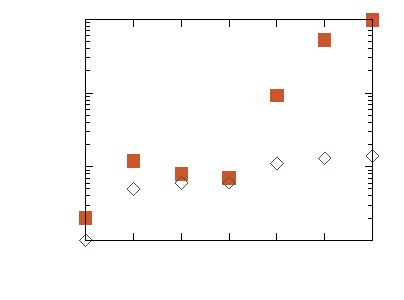
\includegraphics[width={504.00bp},height={144.00bp}]{unhashed-performance-combined}}%
    \gplfronttext
  \end{picture}%
\endgroup
}
  \caption[Comparing the performance of predicate validators.]{Comparing the
    performance of the na\"ive hyperblock scheduling validator without hashing,
    compared to the validator with predicate hashing.  The blocks that are
    tested are manually written and manually scheduled, and are sorted by the
    time taken by the hashed predicated validator to prove the equivalence.}%
  \label{fig:eval:comparison-hashing}
\end{figure}

To assess whether \VericertHyper{} has acceptable compilation times, I also
compare it against Bambu.  Compilation times did not deviate for Bambu, all of
them being around 3s mainly due to long startup costs. \VericertHyper{} compiled
each benchmark in 0.9s, also without much variation, showing that verification
was not overly costly.  As for whether our design decisions led to these
compilation times: I remark that if the \enquote{final-state predicates}
innovation that we introduced in \cref{sec:thirdattempt} is disabled, that none
of the benchmarks compile within a few minutes and eventually the machine runs
out of memory.

To get a better idea of the difference between using the hashed, final-state
predicates compared to the more naïve validator,
\cref{fig:eval:comparison-hashing} shows detailed times of how long validation
took on some hand-crafted examples, that would not time-out the verification for
the naïve validator.  The example test programs differ roughly in the number of
predicates that are present.  This shows that using final-state predicates meant
that validation time stayed mostly constant, whereas the naïve validator quickly
took exponentially more time to validate the same schedule.

\section{RQ5: Effectiveness of Vericert's Correctness Theorem}

\definecolor{fuzzred}{HTML}{f8514f}
\definecolor{fuzzyellow}{HTML}{fee4bf}
\definecolor{fuzzgreen}{HTML}{b2df8a}
\begin{figure}
  \centering
  %\begin{tabular}{cccc}\toprule
  %  \textbf{Passing} & \textbf{Compile time errors} & \textbf{Runtime errors} & \textbf{Total}\\\midrule
  %  40379 (26.00\%) & 114849 (73.97\%) & 39 (0.03\%) & 155267\\\bottomrule
  %\end{tabular}

  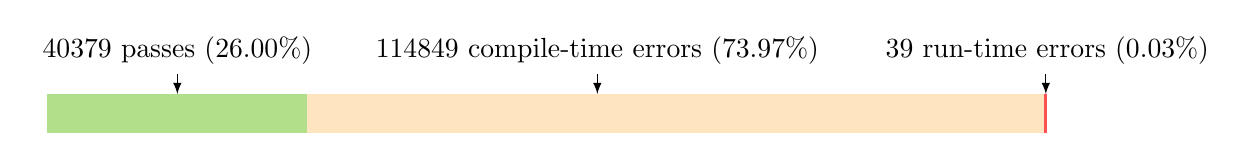
\begin{tikzpicture}[xscale=0.127]
  \draw[-latex] (13,0.5) to (13,0.25);
  \draw[-latex] (55,0.5) to (55,0.25);
  \draw[-latex] (99.85,0.5) to (99.85,0.25);
  \draw[fuzzgreen, line width=5mm] (0,0) to (26.0,0);
  \draw[fuzzyellow, line width=5mm] (26.0,0) to (99.7,0);
  \draw[fuzzred, line width=5mm] (99.7,0) to (100,0);
  \node[anchor=south] at (13,0.5) {40379 passes (26.00\%)};
  \node[anchor=south] at (55,0.5) {114849 compile-time errors (73.97\%)};
  \node[anchor=south] at (100,0.5) {39 run-time errors (0.03\%)};
  \end{tikzpicture}
  \caption{Results of fuzzing \vericert{} using 155267 random C programs generated by Csmith.}\label{tab:fuzzing}
\end{figure}

\begin{quotation}
  \textit{\enquote{Beware of bugs in the above code; I have only proved it
      correct, not tried it.}}\par\hfill -- D. E. Knuth (1977)
\end{quotation}

\noindent To gain further confidence that the Verilog designs generated by
\vericert{} are actually correct, and that the correctness theorem is indeed
effective, I fuzzed \vericert{} using
Csmith~\cite{yang11_findin_under_bugs_c_compil}. \citeauthor{yang11_findin_under_bugs_c_compil}
previously used Csmith in an extensive fuzzing campaign on CompCert and found a
handful of bugs in the unverified parts of that compiler, so it is natural to
explore whether it can find bugs in \vericert{} too. \citet{herklotz21_esrhlst}
have recently used Csmith to fuzz other HLS tools including \legup{}, so I
configured Csmith in a similar way. In addition to the features turned off by
\citeauthor{herklotz21_esrhlst}, I turned off the generation of global variables
and non-32-bit operations. The generated designs were tested by simulating them
and comparing the output value to the results of compiling the test-cases with
GCC 10.3.0.

The results of the fuzzing run are shown in Fig.~\ref{tab:fuzzing}.  Out of
155267 test-cases generated by Csmith, 26\% of them passed, meaning they
compiled without error and resulted in the same final value as GCC. Most of the
test-cases, 73.97\%, failed at compile time.  The most common reasons for this
were unsigned comparisons between integers (\vericert{} requires them to be
signed), and the presence of 8-bit operations (which \vericert{} does not
support, and which I could not turn off due to a limitation in Csmith).  Because
the test-cases generated by Csmith could not be tailored exactly to the C
fragment that \vericert{} supports, such a high compile-time failure rate is
expected. Finally, and most interestingly, there were a total of 39 run-time
failures, which the correctness theorem should be proving impossible.  However,
all 39 of these failures are due to a bug in the pretty-printing of the final
Verilog code, where a logical negation (\texttt{!}) was accidentally used
instead of a bitwise negation (\verb|~|).  Once this bug was fixed, all
test-cases passed.

\section{Summary}

Vericert with hyperblock scheduling seems to generate hardware around the same
cycle count as the hardware generated by Bambu HLS, which is encouraging.
However, due to if-conversion and scheduling sometimes mispredicting the latency
of certain operations, especially predicated operations, the final execution
time of Vericert is $1.57\times$ that of Bambu HLS.  With better latency
estimation, I am confident that this could get closer to unoptimised Bambu HLS.
However, to get closer to optimised Bambu HLS, more optimisations will need to
be implemented.  One important optimisation that is missing from Vericert is
loop scheduling, which would close the gap to Bambu HLS, especially on a
loop-centric benchmark such as \polybench{}.

% \Cref{fig:list-against-hyper-scheduling} shows the final results relative to the base version of Vericert.  First, the relative cycle counts between each tool shows that list scheduling has 0.59$\times$ the number of cycles compared to base Vericert and hyperblock scheduling has 0.56$\times$ the number of cycles compared to base Vericert, showing that scheduling instructions provides a large improvement compared to the total number of cycles of base Vericert.  Bambu with optimisations turned-off has around 0.42$\times$ the number of cycles, and with optimisations has 0.14$\times$ the number of cycles, taking drastically fewer cycles.  One outlier here is the jacobi-1d benchmark, where only optimised Bambu finds a way to reduce the number of cycles.  This is because it is a very small benchmark with a single loop, which cannot be optimised by the scheduling algorithms and requires more advanced loop optimisations such as loop pipelining.

% However, looking at the relative execution time is a bit surprising, because on average, the hyperblock scheduling algorithm only performs as well as base Vericert, whereas the list scheduling algorithm performs much better.  This is because the operation chaining heuristics used did not work consistently for the hyperblock scheduling pass, therefore reducing the maximum operating frequency dramatically in some cases.  This is something that needs to be addressed in the heuristics used to perform the if-conversion, but also in the latency constraints in the scheduler.  Interestingly, however, the output of the list scheduling algorithm is around 14\% faster than unoptimised Bambu.  Again, optimised Bambu optimises the benchmarks much further, but also has a slightly higher maximum frequency, bringing the gap down a bit compared to the total cycle counts.

% Finally, looking at area, list scheduling actually also reduces the area
% compared to base Vericert, which is mainly due to the synthesis tool being
% able to optimise chained operations, such as multiply-accumulate operations,
% further.  However, because of the addition of predicates in hyperblock
% scheduling, the area is similar to base Vericert.  This area is similar to
% unoptimised Bambu, however, optimised Bambu achieves 0.6$\times$ the area.

%%% Local Variables:
%%% mode: latex
%%% TeX-master: "../thesis"
%%% TeX-engine: luatex
%%% End:
